\documentclass[aspectratio=169,11pt]{beamer}  % 11pt: Inter (EAFIT font) is wider than Latin Modern
\usepackage{eafitml}
\usepackage{colortbl}
% scalable big operators (lmex is size-fixed by default)
\DeclareFontFamily{OMX}{lmex}{}
\DeclareFontShape{OMX}{lmex}{m}{n}{<->lmex10}{}
\setbeamerfont{title}{series=\bfseries,size=\Large}
\lstset{columns=flexible}

% ------------------------------------------------------------ local macros
\makeatletter
% frame title + gray subtitle (as in the original slides)
\setbeamertemplate{frametitle}{\vskip0.25em\usebeamerfont{frametitle}\usebeamercolor[fg]{frametitle}\insertframetitle\par
  \ifx\insertframesubtitle\@empty\else\vskip0.1em{\normalfont\footnotesize\color{mlgray}\insertframesubtitle\par}\fi}
\makeatother
% table of contents (same style as sessions 1-2)
\setbeamertemplate{section in toc}{\leavevmode{\color{mlgold}\inserttocsectionnumber.}~\inserttocsection\par}
\setbeamertemplate{subsection in toc}{\leavevmode\leftskip=2.2em\small\mdseries\inserttocsubsection\par}
\setbeamerfont{section in toc}{series=\bfseries,size=\normalsize}

% figure on white page, placed at bbox (38,20)-(413,230) pt
\newcommand{\figframe}[1]{%
  {\setbeamertemplate{background}{\vbox to\paperheight{\vskip20bp\hbox{\hskip38bp\includegraphics[width=375bp,height=210bp]{#1}}\vss}}%
   \begin{frame}[plain]\end{frame}}}
% gold header + light teal body ("Uso práctico", "Ejemplo esperado", ...)
\newtcolorbox{goldbox}[1][]{enhanced,sharp corners,boxrule=0pt,frame hidden,
  colback=mltealbg,colbacktitle=mlgold,coltitle=white,
  fonttitle=\bfseries\small,left=4pt,right=4pt,top=2pt,bottom=2pt,
  toptitle=1pt,bottomtitle=1pt,before skip=4pt,after skip=4pt,title={#1}}
\setbeamersize{text margin left=18.6pt,text margin right=18.6pt}
\newcolumntype{P}[1]{>{\raggedright\arraybackslash}p{#1}}
% table conventions
\arrayrulecolor{mltitle}
\newcommand{\hrow}{\rowcolor{mlcream}}
\newcommand{\Lg}{\fontsize{16}{20}\selectfont}
\newcommand{\bigstate}[1]{\begin{center}\Lg #1\end{center}}
\newcommand{\bigq}[1]{\begin{center}\Lg\bfseries #1\end{center}}

\title[Series de tiempo, forecasting tabular y walk-forward validation]{Series de tiempo, forecasting tabular y walk-forward validation}
\subtitle{Aprendizaje Automático · Sesión 3}
\author[Aprendizaje Automático]{Andrés Vásquez Restrepo\\[2pt]{\normalfont\small\texttt{avasquezr3@eafit.edu.co}}}
\institute{SI7009 - 1 (5553)\\Universidad EAFIT}
\date{2026-2 -- Medellín}
\titlegraphic{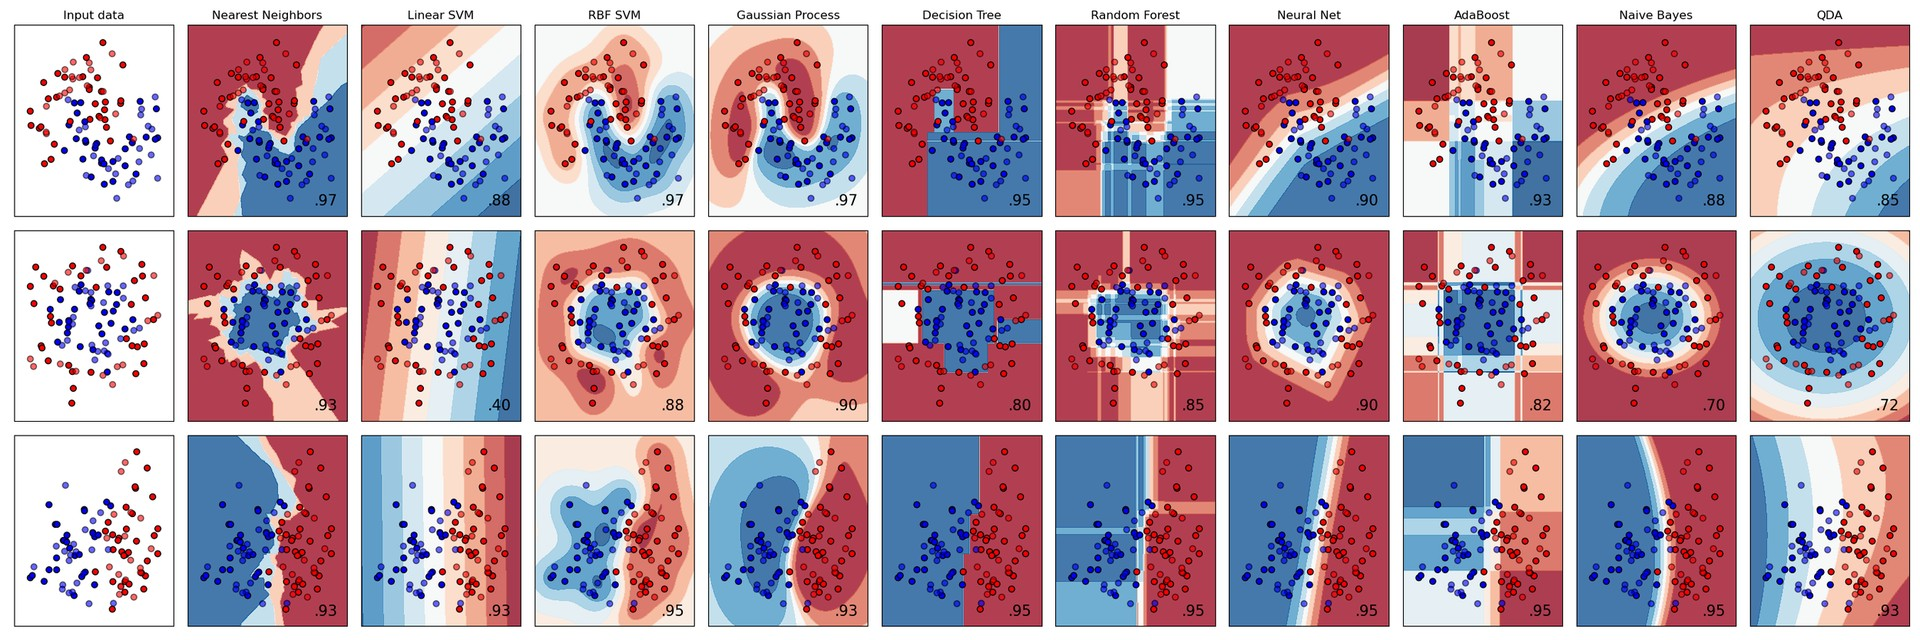
\includegraphics[width=5cm]{figures/img_p001_01.jpg}}

\begin{document}

% ============================================================ p1
\titleframe
\setcounter{framenumber}{1}

% ============================================================ p2
\begin{frame}[t]{Contenido}
\vspace*{-0.3em}
{\setlength{\parskip}{0pt}\tableofcontents}
\end{frame}

% ============================================================ p3
\section{El tiempo cambia el experimento}
\sectionframe{\LARGE El tiempo cambia el experimento}

\begin{frame}{La pregunta central de esta sesión}
\framesubtitle{El problema no es tener fechas; es predecir sin mirar el futuro}
\bigstate{En datos temporales, un score alto no demuestra valor si el experimento permitió mirar el futuro.}
\vspace{0.3em}
\bigq{¿Qué resultado puedo creer si las filas tienen pasado, presente y futuro?}
\vspace{0.3em}
\begin{itemize}
\item El orden define qué información era observable.
\item El horizonte define qué tan lejos queremos predecir.
\item La validación define si el score representa operación real.
\end{itemize}
\end{frame}

\imageframe{figures/img_p005_02.jpg}

\begin{frame}{Lo aprendido antes se vuelve más exigente}
\framesubtitle{La temporalidad tensiona baseline, métrica, split y leakage}
\bigstate{En las sesiones anteriores aprendimos que una mala métrica, un baseline débil o una validación incorrecta pueden engañar.}
\vspace{0.3em}
\bigq{¿El modelo habría tenido esta información en el momento real en que debía predecir?}
\vspace{0.3em}
{\Lg Si la respuesta es no, el resultado puede estar inflado aunque el código sea correcto.\par}
\end{frame}

\begin{frame}{El tiempo rompe la intercambiabilidad}
\framesubtitle{Las filas ya no pueden tratarse como piezas sueltas}
\Lg
\[ y_1,\ y_2,\ \ldots,\ y_t,\ \ldots,\ y_T \]
\vspace{0.3em}
\[ \hat y_{t+h} = f(X_t) \text{ con } X_t \text{ disponible solo hasta } t \]
\begin{itemize}
\item El pasado puede explicar el futuro.
\item El futuro no puede participar en la evidencia usada para evaluar el pasado.
\end{itemize}
\end{frame}

\figframe{figures/img_p008_03.jpg}

\begin{frame}{Chequeo inicial: ¿qué podía saber el modelo?}
\framesubtitle{Antes de entrenar, audite la disponibilidad de información}
\begin{taskbox}[{\large Discusión breve}]
Queremos predecir el volumen de tráfico una hora adelante. Para una predicción hecha a las 8:00 AM, decida qué información es válida.
\end{taskbox}
\begin{enumerate}
\item Volumen observado a las 7:00 AM.
\item Promedio de tráfico entre 8:00 AM y 10:00 AM.
\item Hora del día y día de la semana.
\item Clima reportado después del periodo objetivo.
\item Volumen de la misma hora del día anterior.
\end{enumerate}
Una columna histórica solo es válida si su versión operacional existía antes de la predicción.
\end{frame}

% ============================================================ p10
\section{Antes de modelar: leer la estructura temporal}
\sectionframe{\LARGE Antes de modelar: leer la estructura\\temporal}

\begin{frame}{Una serie de tiempo no es solo una fecha}
\framesubtitle{Es una señal ordenada con memoria, ciclos y posible cambio}
\bigstate{Una serie temporal combina valor, orden, frecuencia, contexto y dependencia histórica.}
\vspace{0.8em}
{\Large\[ y_1,\ y_2,\ \ldots,\ y_t,\ \ldots,\ y_T \]}
{\Lg Si se pierde el \textbf{orden}, también se pierde la estructura que hace posible el \emph{forecasting}.\par}
\end{frame}

\imageframe{figures/img_p012_04.jpg}

\begin{frame}{Componentes básicos de una serie}
\framesubtitle{Antes del modelo, lea la estructura de la señal}
{\Large\[ y_t = T_t + S_t + R_t \]}
\vspace{0.5em}
\begin{columns}[T]
\column{0.32\textwidth} $T_t$: \textbf{tendencia}\\ Cambio lento del nivel.
\column{0.32\textwidth} $S_t$: \textbf{estacionalidad}\\ Patrón repetido.
\column{0.32\textwidth} $R_t$: \textbf{residuo}\\ Lo que queda sin explicar.
\end{columns}
\begin{rulebox}[Cuidado]
La descomposición ayuda a leer tendencia y ciclos; la evidencia predictiva sigue dependiendo de validación hacia adelante.
\end{rulebox}
\end{frame}

\figframe{figures/img_p014_05.jpg}

\begin{frame}{Frecuencia y granularidad}
\framesubtitle{La pregunta cambia si los datos son horarios, diarios o mensuales}
\centering
\begin{tabular}{@{}l P{0.37\textwidth} P{0.37\textwidth}@{}}
\toprule
\hrow \textbf{Frecuencia} & Posibles ciclos & Riesgo frecuente\\
\midrule
\textbf{Horaria} & hora del día, día de la semana & confundir ciclos diarios con ruido\\
\textbf{Diaria} & semana, mes, festivos & ignorar fines de semana y eventos\\
\textbf{Semanal} & mes, trimestre, temporada & tener pocos puntos por ciclo\\
\textbf{Mensual} & año, temporada comercial & sobreinterpretar series cortas\\
\bottomrule
\end{tabular}

\vspace{1.2em}
\textbf{Regla:} La frecuencia define qué \emph{lags}, ventanas, estacionalidades y métricas tienen sentido.
\end{frame}

\begin{frame}{Autocorrelación: memoria estadística}
\framesubtitle{El pasado puede seguir hablando en el presente}
{\Large\[ \rho_k = \operatorname{corr}(y_t,\ y_{t-k}) \]}
\begin{itemize}
\item $\rho_1$ alto sugiere persistencia inmediata.
\item $\rho_{24}$ alto en datos horarios sugiere ciclo diario.
\item Autocorrelación orienta lags y baselines; no prueba causalidad.
\end{itemize}
\begin{goldbox}[Uso práctico]
Si $\rho_{24}$ es alto, $\mathrm{lag}_{24}$ y seasonal naïve merecen probarse antes de entrenar modelos complejos.
\end{goldbox}
\end{frame}

\figframe{figures/img_p017_06.jpg}

\begin{frame}{Estabilidad temporal: cuándo el pasado representa el futuro}
\framesubtitle{Estacionariedad como criterio práctico, no como formalismo central}
\bigstate{La estacionariedad pregunta si el pasado y el futuro obedecen una estructura estadística comparable.}
\begin{itemize}\small
\item Si la media cambia fuertemente, el pasado puede no representar bien el futuro.
\item Si hay tendencia, trabajar con cambios puede estabilizar parte de la señal.
\item Si hay estacionalidad, conviene probar baselines y features estacionales.
\end{itemize}
\bigstate{\textbf{La estabilidad temporal no se asume:} se inspecciona y luego se valida hacia adelante.}
\end{frame}

\begin{frame}{Checklist de diagnóstico antes de modelar}
\framesubtitle{El modelo no debe ser la primera herramienta}
Antes de entrenar, responda
\begin{enumerate}
\item ¿Cuál es la frecuencia real de la serie?
\item ¿Hay huecos, duplicados o cambios de granularidad?
\item ¿Hay tendencia visible?
\item ¿Hay estacionalidad diaria, semanal o anual?
\item ¿La ACF sugiere persistencia o ciclos?
\item ¿El baseline seasonal naïve parece competitivo?
\item ¿El horizonte elegido coincide con la decisión operativa?
\end{enumerate}
\vspace{0.5em}
\begin{center}
Una serie de tiempo se entiende primero como fenómeno; solo después como matriz de entrenamiento.
\end{center}
\end{frame}

% ============================================================ p20
\section{Target temporal, predicción y horizonte}
\sectionframe{\LARGE Target temporal, predicción y\\horizonte}

\begin{frame}{``Predecir tráfico'' no es una formulación completa}
\framesubtitle{Un problema temporal exige coordenadas de tiempo}
\bigstate{Antes de entrenar, una \textbf{formulación temporal} debe fijar qué se predice, desde cuándo, con qué información y a qué horizonte.}
\begin{columns}[T]
\column{0.45\textwidth}
\textbf{Contrato mínimo}
\begin{itemize}
\item ¿Qué variable se predice?
\item ¿Desde qué momento se predice?
\item ¿Qué información está disponible?
\item ¿A cuántos pasos hacia adelante?
\end{itemize}
\column{0.47\textwidth}
\vspace{0.6em}
\begin{rulebox}[Formulación incompleta]
``Predecir demanda'' o ``predecir tráfico'' no alcanza si no define tiempo de predicción, horizonte y disponibilidad.
\end{rulebox}
\end{columns}
\end{frame}

\begin{frame}{La predicción temporal como problema supervisado}
\framesubtitle{El target pertenece al futuro; las features pertenecen al pasado disponible}
{\Large\[ \hat y_{t+h} = f(X_t) \]}
\begin{columns}[T]
\column{0.23\textwidth} $t$\\ Momento en que el sistema debe tomar la predicción.
\column{0.23\textwidth} $h$\\ \textbf{Horizonte:} distancia entre predicción y objetivo.
\column{0.23\textwidth} $X_t$\\ Información conocida hasta $t$.
\column{0.23\textwidth} $y_{t+h}$\\ Valor futuro que queremos estimar.
\end{columns}
\vspace{1em}
\begin{center}
El modelo no predice ``el futuro'' en abstracto: predice una \emph{variable específica}, desde un momento específico $t$, a un horizonte específico $h$.
\end{center}
\end{frame}

\figframe{figures/img_p023_07.jpg}

\begin{frame}{El horizonte cambia la formulación}
\framesubtitle{Un buen modelo a 1 hora no necesariamente sirve a 24 horas}
\centering
\begin{tabular}{@{}l P{0.39\textwidth} P{0.41\textwidth}@{}}
\toprule
\hrow \textbf{Horizonte} & Pregunta operativa & Lectura metodológica\\
\midrule
\textbf{1 hora} & ¿Qué pasará casi inmediatamente? & alta dependencia del estado reciente\\
\textbf{3 horas} & ¿Cómo evoluciona el corto plazo? & empieza a importar la tendencia local\\
\textbf{6 horas} & ¿Qué patrón domina medio día operativo? & pueden aparecer ciclos y cambios de régimen\\
\textbf{24 horas} & ¿Qué ocurrirá en el mismo punto del siguiente día? & la estacionalidad diaria puede ser más importante que el último valor\\
\bottomrule
\end{tabular}

\vspace{0.8em}
No reporte un único \emph{score} como si el desempeño fuera igual para todos los horizontes.
\end{frame}

\begin{frame}{Práctica: complete la formulación temporal}
\framesubtitle{La precisión del lenguaje protege la validez del experimento}
\begin{taskbox}[{\large Ejercicio breve}]
Transforme cada frase vaga en una formulación temporal completa: target, momento de predicción, horizonte e información disponible.
\end{taskbox}
\begin{enumerate}
\item ``Predecir tráfico en la autopista.''
\item ``Predecir demanda de bicicletas.''
\item ``Predecir deterioro respiratorio en monitoreo de pacientes.''
\item ``Predecir ventas para inventario.''
\end{enumerate}
\begin{goldbox}[Ejemplo esperado]
Predecir el volumen de tráfico a las 9:00 AM usando información disponible hasta las 8:00 AM, con horizonte $h=1$ hora.
\end{goldbox}
\end{frame}

\begin{frame}{El caso aplicado debe servir al método, no al revés}
\framesubtitle{Metro será la columna vertebral; los demás datasets cumplen funciones pedagógicas específicas}
\centering\footnotesize
\begin{tabular}{@{}P{0.27\textwidth} P{0.36\textwidth} P{0.30\textwidth}@{}}
\toprule
\hrow \textbf{Dataset} & Por qué sirve & Uso en la sesión\\
\midrule
\textbf{Metro Interstate Traffic Volume} & Tráfico horario, clima, festivos, calendario y estacionalidad diaria & Caso aplicado principal para horizonte, lags, baselines y walk-forward\\
\textbf{Bike Sharing Dataset} & Demanda horaria, clima, calendario, temporada y menor complejidad operativa & Respaldo pedagógico para repetir la metodología en un caso más liviano\\
\textbf{Serie sintética} & Tendencia, ciclo y ruido controlados & Mostrar por qué un random split puede inflar el desempeño temporal\\
\textbf{Dummy manual} & Pocos valores y alineación completamente visible & Enseñar lag, target futuro, horizonte y pérdida de filas sin ruido\\
\bottomrule
\end{tabular}

{\small El \emph{dataset} no se elige por fama; se elige porque permite demostrar decisiones temporales correctas.\par}
\end{frame}

% ============================================================ p27
\subsection{De serie temporal a tabla supervisada}
\sectionframe{\LARGE De serie temporal a tabla supervisada}

\begin{frame}{Forecasting tabular: convertir memoria en features}
\framesubtitle{El objetivo no es ``usar fechas''; es construir filas válidas de predicción}
\Lg
\begin{itemize}
\item Un modelo tabular no entiende una serie temporal por defecto.
\item Debemos convertir pasado disponible en una fila supervisada.
\item \textbf{Fila temporal supervisada:} una fila representa una predicción hecha en $t$, usando información disponible hasta $t$, para estimar un valor futuro $y_{t+h}$.
\item \textbf{Error común:} Crear columnas temporales sin revisar alineación puede producir un dataset elegante pero contaminado.
\end{itemize}
\end{frame}

\imageframe{figures/img_p029_08.jpg}

\begin{frame}{La unidad real de entrenamiento}
\framesubtitle{Cada fila tiene una pregunta temporal específica}
{\Large\[ \mathbf{z}_t = \bigl[y_{t-1},\ y_{t-24},\ \mathrm{rolling}_{24}(t),\ \mathrm{calendar}(t),\ \mathrm{exo}(t)\bigr] \longrightarrow y_{t+h} \]}
\begin{itemize}
\item $\mathbf{z}_t$ contiene solo señales disponibles al momento de predicción.
\item $y_{t-1}$ representa memoria inmediata.
\item $y_{t-24}$ representa una referencia estacional diaria.
\item $\mathrm{exo}(t)$ debe ser una versión externa disponible en $t$, no una observación futura.
\end{itemize}
Cada fila representa una decisión hecha en $t$: qué sabía el sistema y qué futuro debía estimar.
\end{frame}

\begin{frame}{Ejemplo mínimo de alineación}
\framesubtitle{La primera intuición del notebook debe ser manual y visible}
\centering
\begin{tabular}{@{}c c c c P{0.36\textwidth}@{}}
\toprule
\hrow \textbf{Tiempo} & $y_t$ observado & $\mathrm{lag}_1$ & Target $y_{t+1}$ & Lectura\\
\midrule
\textbf{08:00} & 120 & -- & 135 & no hay historia suficiente para $\mathrm{lag}_1$\\
\textbf{09:00} & 135 & 120 & 150 & fila válida para predecir 10:00\\
\textbf{10:00} & 150 & 135 & 142 & fila válida para predecir 11:00\\
\textbf{11:00} & 142 & 150 & -- & no conocemos target futuro al construir evidencia histórica\\
\bottomrule
\end{tabular}

\vspace{1.5em}
Al desplazar \emph{features} y \emph{target}, algunas filas se pierden. Esa pérdida no es un error: es consecuencia de respetar el tiempo.
\end{frame}

\begin{frame}{Una tabla temporal puede estar mal aunque se vea completa}
\framesubtitle{La validez depende de cómo se construyó cada columna}
\begin{columns}[T]
\column{0.47\textwidth}
\textbf{Fila temporal válida}
\begin{itemize}
\item usa valores anteriores a $t$;
\item calcula agregados con ventana histórica;
\item incorpora calendario conocido;
\item usa variables exógenas disponibles antes de decidir.
\end{itemize}
\column{0.47\textwidth}
\textbf{Fila temporal contaminada}
\begin{itemize}
\item usa $y_{t+h}$ directa o indirectamente;
\item calcula promedios con datos futuros;
\item normaliza usando todo el dataset;
\item incluye variables publicadas después del evento.
\end{itemize}
\end{columns}
\begin{rulebox}[Regla metodológica]
La validez de una feature depende de su disponibilidad operacional, no de su presencia en el archivo.
\end{rulebox}
\end{frame}

% ============================================================ p33
\subsection{Features temporales válidas}
\sectionframe{\LARGE Features temporales válidas}

\begin{frame}{Lags y rolling windows convierten memoria en evidencia}
\framesubtitle{Cada feature temporal debe representar pasado disponible}
\bigstate{Un modelo tabular solo puede usar memoria temporal si se la entregamos como features correctamente alineadas.}
\begin{columns}[T]
\column{0.47\textwidth}
\textbf{Lags}
\begin{itemize}
\item capturan memoria puntual;
\item conectan el valor actual con valores anteriores;
\item sirven como referencias históricas directas.
\end{itemize}
\column{0.47\textwidth}
\textbf{Rolling windows}
\begin{itemize}
\item resumen comportamiento reciente;
\item capturan nivel local y variabilidad;
\item suavizan ruido sin mirar el futuro.
\end{itemize}
\end{columns}
\end{frame}

\figframe{figures/img_p035_09.jpg}

\begin{frame}{Lags y ventanas: fórmulas que solo valen si miran al pasado}
\framesubtitle{La alineación importa más que el nombre de la columna}
{\Large
\[ \mathrm{lag}_k(t) = y_{t-k} \]
\[ \mathrm{rolling\_mean}_w(t) = \frac{1}{w}\sum_{i=1}^{w} y_{t-i} \]}
\Lg
Un \emph{lag} trae un punto del pasado. Una \emph{rolling window} resume una ventana histórica. Ambos son válidos solo si no incluyen valores futuros respecto al momento de predicción.
\end{frame}

\begin{frame}{Feature temporal válida vs feature contaminada}
\framesubtitle{El nombre de la columna no garantiza la validez}
\centering
\begin{tabular}{@{}l P{0.36\textwidth} P{0.37\textwidth}@{}}
\toprule
\hrow \textbf{Feature} & Válida si\ldots & Contaminada si\ldots\\
\midrule
$\mathrm{lag}_1$ & usa un valor observado antes de predecir & se construye con el target futuro desplazado al revés\\
$\mathrm{lag}_{24}$ & representa la misma hora del día anterior disponible & usa una medición corregida después del periodo objetivo\\
$\mathrm{rolling\_mean}_{24}$ & promedia solo valores anteriores al momento $t$ & incluye $y_t$, $y_{t+1}$ o valores posteriores sin justificación operacional\\
$\mathrm{rolling\_std}_{24}$ & resume variabilidad histórica reciente & se calcula sobre toda la serie antes del split temporal\\
\bottomrule
\end{tabular}

\raggedright
Una \emph{feature} temporal debe poder reconstruirse en producción usando solamente lo que el sistema sabía en ese momento.
\end{frame}

\begin{frame}{El calendario es válido, pero debe codificarse como ciclo}
\framesubtitle{Disponibilidad y geometría temporal son problemas distintos}
\bigstate{Hora, día de la semana, mes y festivos pueden ser features legítimas porque se conocen antes de predecir.}
\begin{columns}[T]
\column{0.4\textwidth}
\textbf{Señales conocidas}
\begin{itemize}
\item hora del día;
\item día de la semana;
\item fin de semana;
\item mes o temporada;
\item festivo programado.
\end{itemize}
\column{0.55\textwidth}
\vspace{0.8em}
\begin{rulebox}[Cuidado]
Que una variable sea conocida no garantiza que su codificación preserve la geometría temporal del fenómeno.
\end{rulebox}
\end{columns}
\end{frame}

\figframe{figures/img_p039_10.jpg}

\begin{frame}{La hora no vive en una recta: vive en un ciclo}
\framesubtitle{23:00 y 00:00 están cerca, aunque sus números parezcan lejanos}
\vspace{1em}
{\Large\[ \mathrm{hour}_{\sin} = \sin\!\left(\frac{2\pi\cdot \mathrm{hour}}{24}\right) \qquad \mathrm{hour}_{\cos} = \cos\!\left(\frac{2\pi\cdot \mathrm{hour}}{24}\right) \]}
\begin{columns}[T]
\column{0.47\textwidth}
\textbf{Codificación lineal}
\begin{itemize}
\item $23$ y $0$ parecen muy distantes;
\item impone una frontera artificial al ciclo;
\item puede confundir patrones nocturnos.
\end{itemize}
\column{0.47\textwidth}
\textbf{Codificación cíclica}
\begin{itemize}
\item preserva cercanía circular;
\item representa periodicidad;
\item facilita aprender patrones diarios.
\end{itemize}
\end{columns}
\end{frame}

\begin{frame}{Qué representa cada variable temporal}
\framesubtitle{No toda variable de calendario aporta el mismo tipo de señal}
\centering
\begin{tabular}{@{}l P{0.33\textwidth} P{0.33\textwidth}@{}}
\toprule
\hrow \textbf{Variable} & Qué puede capturar & Codificación razonable\\
\midrule
\textbf{Hora del día} & ciclos de congestión, demanda o actividad & seno/coseno de 24 horas\\
\textbf{Día de la semana} & diferencia entre lunes, viernes y fin de semana & categórica o seno/coseno semanal\\
\textbf{Mes} & estacionalidad anual o patrones de temporada & seno/coseno anual o categórica\\
\textbf{Festivo} & cambios programados en comportamiento & indicador binario conocido antes de predecir\\
\bottomrule
\end{tabular}

\vspace{0.6em}
\raggedright
La variable temporal debe representar una hipótesis sobre el fenómeno, no solo aumentar el número de columnas.
\end{frame}

\begin{frame}{Calendario válido, variable externa dudosa}
\framesubtitle{No todo lo que tiene fecha estaba disponible al decidir}
\begin{taskbox}[{\large Discusión breve}]
Para una predicción hecha a las 8:00 AM, clasifique cada señal como válida, dudosa o contaminada.
\end{taskbox}
\begin{enumerate}
\item Hora del día de la predicción.
\item Día de la semana de la predicción.
\item Indicador de festivo ya conocido en calendario.
\item Clima observado oficialmente a las 10:00 AM.
\item Pronóstico climático disponible antes de las 8:00 AM.
\end{enumerate}
Una variable externa es válida solo si su versión operacional estaba disponible antes del momento de predicción.
\end{frame}

% ============================================================ p43
\section{Antes del modelo: demostrar que el pasado simple no basta}
\sectionframe{\LARGE Antes del modelo: demostrar que el\\pasado simple no basta}

\begin{frame}{Un baseline temporal no es un modelo ridículo}
\framesubtitle{A veces el pasado inmediato o estacional es un competidor fuerte}
\bigstate{Antes de defender un modelo complejo, debemos probar si una \textbf{regla temporal simple} ya resuelve buena parte del problema.}
\begin{itemize}
\item \textbf{Muchas series tienen persistencia:} el último valor observado ya informa bastante.
\item \textbf{Muchas series tienen ciclos:} la misma hora del día anterior puede ser una referencia fuerte.
\item Los promedios recientes pueden ser robustos cuando la serie tiene ruido local.
\end{itemize}
\begin{rulebox}[Criterio de clase]
Un modelo temporal sofisticado que no supera un baseline temporal honesto no merece una defensa fuerte.
\end{rulebox}
\end{frame}

\imageframe{figures/img_p045_11.jpg}

\begin{frame}{Tres referencias temporales obligatorias}
\framesubtitle{Persistencia, estacionalidad y suavizado reciente}
\begin{center}\Large
\textbf{Naïve:}\quad $\hat y_{t+h} = y_t$\\[1em]
\textbf{Seasonal naïve:}\quad $\hat y_{t+h} = y_{t+h-s}$\\
con $s = 24$ para ciclo diario horario\\[0.5em]
\textbf{Moving average:}\quad $\displaystyle \hat y_{t+h} = \frac{1}{w}\sum_{i=0}^{w-1} y_{t-i}$
\end{center}
\vspace{-0.3em}
Estas reglas no intentan ser inteligentes: responden si el modelo agrega valor frente a memoria, ciclo y nivel reciente.
\end{frame}

\begin{frame}{Cuándo cada baseline pone presión real}
\framesubtitle{El baseline correcto depende de la estructura temporal dominante}
\centering
\begin{tabular}{@{}l P{0.35\textwidth} P{0.35\textwidth}@{}}
\toprule
\hrow \textbf{Baseline} & Es fuerte cuando\ldots & Puede fallar cuando\ldots\\
\midrule
\textbf{Naïve} & la serie tiene alta persistencia y cambia lentamente & hay cambios bruscos o ciclos fuertes\\
\textbf{Seasonal naïve} & existe patrón diario, semanal o mensual estable & el ciclo cambia por eventos, clima o régimen\\
\textbf{Moving average} & el nivel reciente resume bien el estado operativo & suaviza demasiado picos, congestión o eventos raros\\
\bottomrule
\end{tabular}

\vspace{1.2em}
En tráfico horario, el último valor puede ser útil; la misma hora del día anterior puede ser más útil; el promedio móvil puede estabilizar ruido.
\end{frame}

\begin{frame}{Práctica: elija un baseline temporal}
\framesubtitle{La elección del baseline revela qué estructura cree que domina}
\begin{taskbox}[{\large Discusión breve}]
Para cada caso, proponga el primer baseline que usaría y explique qué hipótesis temporal está probando.
\end{taskbox}
\begin{enumerate}
\item Volumen de tráfico una hora adelante.
\item Demanda energética para mañana a la misma hora.
\item Ventas diarias con alta variación de fin de semana.
\item Monitoreo fisiológico con mediciones frecuentes y tendencia reciente.
\end{enumerate}
Si el problema del PI tiene tiempo, el baseline debe reflejar memoria, estacionalidad o nivel reciente antes de entrenar modelos complejos.
\end{frame}

% ============================================================ p49
\subsection{Random split: cuando el score puede mentir}
\sectionframe{\LARGE Random split: cuando el score puede\\mentir}

\begin{frame}{Random split puede ser una trampa temporal}
\framesubtitle{El problema no es el método en abstracto; es usarlo donde rompe la operación real}
\bigstate{En forecasting, entrenar con observaciones futuras y validar en observaciones pasadas puede inflar el desempeño porque valida en condiciones más fáciles que la operación real.}
\begin{columns}[T]
\column{0.45\textwidth}
\textbf{Qué parece hacer}\\
Separar datos de forma aleatoria para estimar desempeño con train y validación.
\column{0.47\textwidth}
\vspace{0.3em}
\begin{rulebox}[Qué puede romper]
La dirección real del problema: en operación, el modelo nunca entrena con el futuro para predecir el pasado.
\end{rulebox}
\end{columns}
\end{frame}

\imageframe{figures/img_p051_12.jpg}

\begin{frame}{Qué significa contaminación temporal}
\framesubtitle{El futuro no debe entrenar el modelo que evalúa el pasado}
{\Large\[ \exists\, t_i \in D_{\mathrm{train}},\ \exists\, t_j \in D_{\mathrm{val}} \quad \text{tal que} \quad t_i > t_j \]}
\begin{rulebox}[{\large Lectura}]
\Lg Hay al menos una fila de train ubicada después de una fila de validación.
\end{rulebox}
\bigstate{El score puede subir no porque el modelo sea mejor, sino porque el experimento fue más fácil.}
\end{frame}

\begin{frame}{Tres formas de separar datos temporales}
\framesubtitle{No todas responden la misma pregunta experimental}
\centering
\begin{tabular}{@{}l P{0.34\textwidth} P{0.36\textwidth}@{}}
\toprule
\hrow \textbf{Esquema} & Qué hace & Riesgo o utilidad\\
\midrule
\textbf{Random split} & mezcla observaciones de distintos momentos & puede inflar desempeño si hay dependencia temporal\\
\textbf{Temporal holdout} & entrena en pasado y valida en un bloque futuro & simple, útil y más cercano a operación real\\
\textbf{Walk-forward} & repite la evaluación avanzando en el tiempo & estima desempeño de forma más robusta y operacional\\
\bottomrule
\end{tabular}
\vspace{0.8em}
\begin{rulebox}[Regla]
Para forecasting temporal, el split debe responder: ``¿cómo habría funcionado el modelo si realmente se hubiera usado en ese momento?''.
\end{rulebox}
\end{frame}

\begin{frame}{Práctica: diagnostique el split}
\framesubtitle{Antes de mirar la métrica, mire el flujo del tiempo}
\begin{taskbox}[{\large Discusión breve}]
Decida si cada protocolo es defendible para forecasting de tráfico horario.
\end{taskbox}
\begin{enumerate}
\item Mezclar aleatoriamente todas las horas de 2012 a 2018 y validar con el 20\,\%.
\item Entrenar con 2012--2016 y validar con 2017.
\item Ajustar el escalador con todos los años y luego hacer un split temporal.
\item Entrenar en enero--marzo y validar en abril, repitiendo el proceso con ventanas que avanzan.
\end{enumerate}
\begin{goldbox}[Respuesta esperada]
Un protocolo no es válido porque produzca números; es válido si reproduce la disponibilidad de información que existiría en operación.
\end{goldbox}
\end{frame}

% ============================================================ p55
\subsection{Walk-forward validation: evaluar como si el modelo operara en el tiempo}
\sectionframe{\LARGE Walk-forward validation: evaluar\\como si el modelo operara en el\\tiempo}

\begin{frame}{Validar hacia adelante}
\framesubtitle{Entrenar con pasado, validar en futuro y repetir}
\bigstate{Walk-forward validation simula decisiones sucesivas: entrenar con historia disponible, predecir el siguiente bloque y repetir.}
\begin{itemize}\small
\item El modelo se entrena con historia disponible.
\item Predice un bloque futuro.
\item El origen de predicción avanza.
\item El desempeño se resume sobre varios bloques temporales.
\end{itemize}
\bigstate{La validación temporal pregunta: ¿qué habría pasado si el modelo se hubiera usado en ese momento?}
\end{frame}

\imageframe{figures/img_p057_13.jpg}

\begin{frame}{La restricción cronológica del fold}
\framesubtitle{Cada validación debe estar después de su entrenamiento}
\Large
\begin{gather*}
D^{(k)}_{\mathrm{train}} = \bigl\{(X_t, y_{t+h}) : t \le T_k\bigr\}\\[0.6em]
D^{(k)}_{\mathrm{val}} = \bigl\{(X_t, y_{t+h}) : T_k < t \le T_{k+1}\bigr\}\\[0.6em]
\max\Bigl(t \in D^{(k)}_{\mathrm{train}}\Bigr) < \min\Bigl(t \in D^{(k)}_{\mathrm{val}}\Bigr)
\end{gather*}
\normalsize
\begin{center}
En cada fold, el entrenamiento termina antes de que empiece la validación. Esa desigualdad protege la dirección real del tiempo.
\end{center}
\end{frame}

\begin{frame}{El score final resume varios futuros evaluados}
\framesubtitle{Walk-forward no produce una sola validación cómoda}
{\Large\[ \widehat{E}_{\mathrm{WF}} = \frac{1}{K}\sum_{k=1}^{K} E\Bigl(D^{(k)}_{\mathrm{val}}\Bigr) \]}
\begin{itemize}
\item $K$: número de cortes temporales evaluados.
\item $E(D^{(k)}_{\mathrm{val}})$: error del fold $k$ en un bloque futuro.
\item $\widehat{E}_{\mathrm{WF}}$: desempeño promedio bajo simulación temporal repetida.
\end{itemize}
\begin{center}
El score final es el promedio de errores futuros en varios cortes temporales, no una medición aislada.
\end{center}
\end{frame}

\begin{frame}{Variantes útiles de validación temporal}
\framesubtitle{La decisión depende de historia disponible, estabilidad y costo computacional}
\centering
\begin{tabular}{@{}l P{0.33\textwidth} P{0.33\textwidth}@{}}
\toprule
\hrow \textbf{Esquema} & Cómo entrena & Cuándo tiene sentido\\
\midrule
\textbf{Holdout temporal} & un bloque pasado para train y un bloque futuro para validación & primera comparación simple y clara\\
\textbf{Ventana expansiva} & cada fold acumula más historia antes de validar el siguiente bloque & cuando más historia suele aportar señal útil\\
\textbf{Ventana deslizante} & cada fold usa solo una ventana reciente de longitud fija & cuando los patrones antiguos pueden dejar de representar el presente\\
\bottomrule
\end{tabular}

\vspace{0.4em}
No existe una única validación temporal universal: debe corresponder al uso real, al horizonte y a la estabilidad del fenómeno.
\end{frame}

\begin{frame}{Embargo: una separación cuando hay riesgo de vecindad}
\framesubtitle{No todo fold cronológico queda automáticamente limpio}
\bigstate{Un embargo deja una brecha temporal entre train y validación para reducir contaminación por ventanas solapadas, labels futuros o eventos cercanos.}
{\Large\[ \max(t_{\mathrm{train}}) + g < \min(t_{\mathrm{val}}) \]}
\begin{itemize}\small
\item $g$: tamaño de la brecha temporal.
\item Si $g = 24$ en datos horarios, se deja un día de separación.
\item Útil si las features usan ventanas largas o labels futuros.
\item No reemplaza una mala formulación: solo agrega protección.
\end{itemize}
\end{frame}

\begin{frame}{Práctica: diseñe el protocolo}
\framesubtitle{El split debe ser una decisión defendible, no una línea de código por costumbre}
\begin{taskbox}[{\large Escenario}]
Tiene datos horarios de tráfico entre 2012 y 2018. Quiere predecir una hora adelante y comparar un baseline seasonal naïve, Ridge Regression e HistGradientBoostingRegressor.
\end{taskbox}
\textbf{Defina:}
\begin{enumerate}
\item tamaño del bloque inicial de entrenamiento;
\item tamaño del bloque de validación;
\item si usaría ventana expansiva o deslizante;
\item si necesita embargo;
\item qué métrica reportaría por fold;
\item cómo resumiría el desempeño final.
\end{enumerate}
\end{frame}

% ============================================================ p63
\subsection{Temporal leakage: auditoría del pipeline completo}
\sectionframe{\LARGE Temporal leakage: auditoría del\\pipeline completo}

\begin{frame}{Leakage temporal no siempre parece leakage}
\framesubtitle{No basta con quitar el target futuro}
\bigstate{Temporal leakage ocurre cuando el pipeline usa información que no estaría disponible en el momento real de predicción.}
\begin{itemize}\small
\item Puede entrar por features que miran hacia adelante.
\item Puede entrar por preprocessing ajustado con toda la serie.
\item Puede entrar por variables externas publicadas tarde.
\item Puede entrar por folds que mezclan futuro y pasado.
\end{itemize}
\begin{center}
La pregunta no es \textbf{``¿la columna existe?''}, sino \textbf{``¿el sistema la conocía antes de predecir?''}.
\end{center}
\end{frame}

\imageframe{figures/img_p065_14.jpg}

\begin{frame}{Cinco rutas comunes de leakage temporal}
\framesubtitle{El futuro puede entrar por features, preprocessing o validación}
\centering\small
\begin{tabular}{@{}l P{0.32\textwidth} P{0.32\textwidth}@{}}
\toprule
\hrow \textbf{Ruta} & Qué parece hacer & Por qué contamina\\
\midrule
\textbf{Rolling mal alineado} & calcula una media móvil suave & incluye $y_t$, $y_{t+1}$ o valores posteriores\\
\textbf{Escalamiento global} & normaliza todas las filas antes del split & aprende estadísticas del futuro\\
\textbf{Imputación global} & llena faltantes con toda la serie & usa distribución posterior al momento de predicción\\
\textbf{Variable externa tardía} & agrega clima, reporte o evento observado después & la señal no existía al decidir\\
\textbf{Folds mezclados} & valida en pasado y entrena con futuro & rompe la dirección operacional del forecasting\\
\bottomrule
\end{tabular}

\vspace{0.6em}
El leakage puede ocurrir antes del modelo. Por eso se audita el pipeline completo, no solo el estimador.
\end{frame}

\begin{frame}{La regla formal: disponibilidad antes de $t$}
\framesubtitle{Una feature es válida si pertenece al conjunto de información disponible}
\Large
\begin{align*}
x_j(t) \in \mathcal{I}_t \quad &\Longrightarrow \quad x_j(t) \text{ es candidata válida}\\[0.8em]
x_j(t) \notin \mathcal{I}_t \quad &\Longrightarrow \quad x_j(t) \text{ introduce riesgo de leakage}
\end{align*}
\normalsize
\begin{defbox}[$\mathcal{I}_t$]
Conjunto de información que el sistema podía conocer antes o en el momento operativo de predicción $t$, según la definición del problema.
\end{defbox}
\end{frame}

\begin{frame}{Práctica: audite el pipeline temporal}
\framesubtitle{Un buen score no rescata un flujo contaminado}
\begin{taskbox}[{\large Escenario}]
Un equipo predice tráfico una hora adelante y reporta bajo MAE. Antes de creer el resultado, audite estas decisiones.
\end{taskbox}
\begin{enumerate}
\item Calculó $\mathrm{rolling\_mean}_{24}$ con una ventana centrada.
\item Ajustó \texttt{StandardScaler} usando todo el dataset histórico.
\item Usó el pronóstico climático disponible antes de la hora de predicción.
\item Separó train en 2012--2016 y validación en 2017.
\item Seleccionó features mirando el desempeño sobre el bloque final de test.
\end{enumerate}
\begin{center}
Primero se audita disponibilidad y protocolo; después se interpreta el score.
\end{center}
\end{frame}

% ============================================================ p69
\section{Medir error no basta: hay que interpretarlo contra tiempo y baseline}
\sectionframe{\LARGE Medir error no basta: hay que\\interpretarlo contra tiempo y baseline}

\begin{frame}{Un error bajo no siempre significa un modelo útil}
\framesubtitle{La métrica debe leerse junto al baseline, el horizonte y la validación}
\bigstate{En forecasting, el error no se interpreta solo: se interpreta contra una referencia temporal y bajo un horizonte específico.}
\begin{columns}[T]
\column{0.45\textwidth}
\textbf{Una métrica útil debe decir}
\begin{itemize}
\item cuánto nos equivocamos;
\item en qué unidades;
\item si castigamos errores grandes;
\item si superamos un baseline temporal.
\end{itemize}
\column{0.47\textwidth}
\vspace{0.4em}
\begin{rulebox}[Cuidado]
Un MAE aparentemente bajo puede ser mediocre si el seasonal naïve logra lo mismo con una regla simple.
\end{rulebox}
\end{columns}
\end{frame}

\begin{frame}{MAE y RMSE: dos lecturas del error}
\framesubtitle{Unidades interpretables vs penalización de errores grandes}
\begin{columns}[T]
\column{0.47\textwidth}
{\Large\[ \mathrm{MAE} = \frac{1}{n}\sum_{i=1}^{n} |y_i - \hat y_i| \]}
\textbf{MAE}
\begin{itemize}
\item está en unidades del target;
\item es fácil de comunicar;
\item resume error típico absoluto.
\end{itemize}
\column{0.49\textwidth}
{\Large\[ \mathrm{RMSE} = \sqrt{\frac{1}{n}\sum_{i=1}^{n} (y_i - \hat y_i)^2} \]}
\textbf{RMSE}
\begin{itemize}
\item castiga más los errores grandes;
\item es sensible a picos;
\item puede ser útil si los desvíos extremos son costosos.
\end{itemize}
\end{columns}
\end{frame}

\imageframe{figures/img_p072_15.jpg}

\begin{frame}{MASE (Error Absoluto Medio Escalado): escalar el error con una referencia temporal}
\framesubtitle{La pregunta es: ¿mejoro una predicción naïve?}
{\Large\[ \mathrm{MASE} = \frac{\frac{1}{n}\sum_{i=1}^{n} |y_i - \hat y_i|}{\frac{1}{T_{\mathrm{train}}-1}\sum_{t=2}^{T_{\mathrm{train}}} |y_t - y_{t-1}|} \]}
\begin{itemize}
\item El numerador mide el error absoluto promedio del modelo.
\item El denominador debe calcularse con una referencia naïve sobre el periodo de entrenamiento.
\item Si el baseline relevante es seasonal naïve, conviene reportar una variante estacional de MASE.
\end{itemize}
\end{frame}

\begin{frame}{Cómo interpretar MASE}
\framesubtitle{Un modelo complejo debe demostrar valor frente a una regla simple}
\centering\large
\begin{tabular}{@{}c P{0.6\textwidth}@{}}
\toprule
\hrow \textbf{Valor} & Interpretación\\
\midrule
$\mathrm{MASE} < 1$ & el modelo mejora al baseline naïve\\
$\mathrm{MASE} \approx 1$ & el modelo se comporta similar al baseline\\
$\mathrm{MASE} > 1$ & el modelo es peor que una predicción naïve\\
\bottomrule
\end{tabular}

\vspace{1em}
MASE contextualiza el error: no pregunta solo ``cuánto me equivoqué'', sino ``qué tan bueno soy frente a una predicción simple''.
\end{frame}

\begin{frame}{MAPE y sMAPE: útiles con cautela}
\framesubtitle{Error Porcentual Absoluto Medio}
\bigstate{El porcentaje puede parecer intuitivo y aun así engañar. El error porcentual no siempre representa bien el costo operativo.}
\begin{itemize}\small
\item MAPE divide por el valor real; si el valor es bajo o cercano a cero, puede explotar.
\item No todos los problemas tienen un cero con sentido operativo.
\item Un error del 10\,\% puede ser tolerable o grave según el volumen absoluto y la decisión.
\end{itemize}
\begin{rulebox}[Regla de esta sesión]
MAE, RMSE y MASE serán centrales. MAPE/sMAPE quedan como cautela metodológica, no como eje.
\end{rulebox}
\end{frame}

\begin{frame}{Práctica: ¿qué métrica usaría?}
\framesubtitle{La elección de métrica depende de la decisión que se quiere defender}
\begin{taskbox}[{\large Discusión breve}]
Para cada situación, elija la métrica principal y explique qué lectura agregaría con las otras métricas.
\end{taskbox}
\begin{enumerate}
\item Tráfico horario: el equipo operativo necesita entender el error típico en vehículos.
\item Energía: los errores extremos pueden causar sobrecosto alto.
\item Inventario: se quiere demostrar que el modelo supera una regla naïve.
\item Monitoreo fisiológico: un error grande aislado puede ser clínicamente relevante.
\end{enumerate}
\begin{goldbox}[Respuesta esperada]
MAE comunica magnitud típica; RMSE revela sensibilidad a picos; MASE responde si el modelo supera una referencia temporal simple.
\end{goldbox}
\end{frame}

% ============================================================ p77
\subsection{Evaluación multi-horizon}
\sectionframe{\LARGE Evaluación multi-horizon}

\begin{frame}{Un modelo no tiene un único desempeño temporal}
\framesubtitle{El horizonte cambia la dificultad, la señal útil y la decisión}
\bigstate{Predecir 1 hora adelante no es el mismo problema que predecir 24 horas adelante.}
\begin{columns}[T]
\column{0.47\textwidth}
\textbf{Horizonte corto}
\begin{itemize}
\item depende más del estado reciente;
\item los lags cercanos suelen ser fuertes;
\item puede ser útil para decisiones operativas inmediatas.
\end{itemize}
\column{0.47\textwidth}
\textbf{Horizonte largo}
\begin{itemize}
\item aumenta incertidumbre;
\item puede depender más de ciclos;
\item puede requerir otra formulación o features distintas.
\end{itemize}
\end{columns}
\bigstate{No esconda varios horizontes dentro de un solo número si la decisión operativa depende del tiempo hacia adelante.}
\end{frame}

\figframe{figures/img_p079_16.jpg}

\begin{frame}{Evaluar por horizonte}
\framesubtitle{El error debe indexarse por la distancia al futuro}
\Large
\[ \widehat{y}_{t+h} = f_h(X_t) \qquad h \in \{1, 3, 6, 24\} \]
\[ E_h = \frac{1}{n_h}\sum_{i=1}^{n_h} L(y_{t_i+h}, \widehat{y}_{t_i+h}) \]
\normalsize
\begin{itemize}
\item $h$: horizonte de predicción.
\item $f_h$: modelo o formulación usada para ese horizonte.
\item $L(\cdot)$: pérdida o métrica de error, por ejemplo MAE.
\item $E_h$: error estimado específicamente para el horizonte $h$.
\end{itemize}
\end{frame}

\begin{frame}{Cómo cambia la utilidad por horizonte}
\framesubtitle{La métrica debe leerse con la decisión que habilita}
\centering
\begin{tabular}{@{}l P{0.39\textwidth} P{0.40\textwidth}@{}}
\toprule
\hrow \textbf{Horizonte} & Señal que suele dominar & Decisión que puede soportar\\
\midrule
\textbf{1 hora} & estado reciente, $\mathrm{lag}_1$, tendencia local & gestión inmediata de congestión o alertas operativas\\
\textbf{3 horas} & persistencia y cambios de corto plazo & planeación táctica en el mismo bloque del día\\
\textbf{6 horas} & ciclos diarios parciales y contexto externo & anticipación de carga operativa en media jornada\\
\textbf{24 horas} & estacionalidad diaria, calendario y patrones recurrentes & planeación del día siguiente o inventario de recursos\\
\bottomrule
\end{tabular}

\vspace{0.3em}\raggedright
Un modelo puede ser defendible para $h=1$ y no defendible para $h=24$. Esa diferencia debe aparecer en el reporte.
\end{frame}

\begin{frame}{Práctica: lea resultados por horizonte}
\framesubtitle{El ganador puede depender del futuro que realmente importa}
\begin{taskbox}[{\large Escenario}]
Dos modelos tienen el siguiente comportamiento: Modelo A gana claramente en MAE para 1 hora; Modelo B es más estable para 6 y 24 horas. El equipo operativo necesita planear recursos para el día siguiente.
\end{taskbox}
\textbf{Discuta:}
\begin{enumerate}
\item ¿Cuál modelo defendería para operación inmediata?
\item ¿Cuál modelo defendería para planeación del día siguiente?
\item ¿Qué baseline temporal debe aparecer en la comparación?
\item ¿Qué reportaría además del promedio global?
\end{enumerate}
La decisión no se toma por ``el mejor modelo'' en abstracto, sino por el modelo que mejora el horizonte que la operación necesita.
\end{frame}

% ============================================================ p83
\section{El modelo entra cuando el experimento ya es defendible}
\sectionframe{\LARGE El modelo entra cuando el\\experimento ya es defendible}

\begin{frame}{Primero formulación, después complejidad}
\framesubtitle{Ridge y HGBR compiten contra baselines bajo validación temporal}
\bigstate{En esta sesión, el objetivo no es probar muchas librerías: es comparar modelos tabulares bajo un protocolo temporal correcto.}
\begin{columns}[T]
\column{0.37\textwidth}
\textbf{Antes del modelo}
\begin{itemize}
\item target temporal;
\item horizonte;
\item features válidas;
\item baselines temporales;
\item walk-forward validation.
\end{itemize}
\column{0.57\textwidth}
\vspace{0.6em}
\begin{rulebox}[Después del modelo]
Si el modelo gana, debe ganar contra una referencia honesta, sin leakage y en el horizonte que importa.
\end{rulebox}
\end{columns}
\end{frame}

\begin{frame}{Dos modelos canónicos para esta sesión}
\framesubtitle{Un baseline supervisado interpretable y un modelo tabular flexible}
\vspace{1.5em}
\begin{center}\Lg
Ridge Regression: \qquad $\hat y = \beta_0 + X\beta$ \quad con regularización
\end{center}
\vspace{0.5em}
\begin{columns}[T]
\column{0.47\textwidth}
\textbf{Ridge}
\begin{itemize}
\item referencia supervisada simple;
\item útil para detectar señal lineal;
\item fácil de explicar y comparar.
\end{itemize}
\column{0.47\textwidth}
\textbf{HistGradientBoostingRegressor}
\begin{itemize}
\item captura no linealidad;
\item maneja interacciones;
\item funciona bien en datos tabulares si las features temporales son válidas.
\end{itemize}
\end{columns}
\end{frame}

\figframe{figures/img_p086_17.jpg}

% ============================================================ p87
\subsection{Mapa de modelos temporales: extensión con control metodológico}
\sectionframe{\LARGE Mapa de modelos temporales:\\extensión con control metodológico}

\imageframe{figures/img_p088_18.jpg}

\begin{frame}{Tres familias, una misma regla de credibilidad}
\framesubtitle{Todo modelo debe competir bajo el mismo protocolo temporal}
\begin{center}\large
Clásico, ML tabular o red neuronal: todos deben competir bajo el mismo target, horizonte, baseline, validación y control de leakage.
\end{center}
\vspace{-0.4em}
\centering\large
\begin{tabular}{@{}l P{0.52\textwidth}@{}}
\toprule
\hrow \textbf{Familia} & Pregunta correcta\\
\midrule
\textbf{ARIMA / SARIMA} & ¿la estructura temporal simple explica suficiente?\\
\textbf{ML tabular} & ¿features históricas válidas mejoran los baselines?\\
\textbf{NN temporal} & ¿la secuencia aporta más valor que el aumento de complejidad?\\
\bottomrule
\end{tabular}
\end{frame}

\figframe{figures/img_p090_19.jpg}

\begin{frame}[plain]
\begin{columns}[c]
\column{0.5\paperwidth}
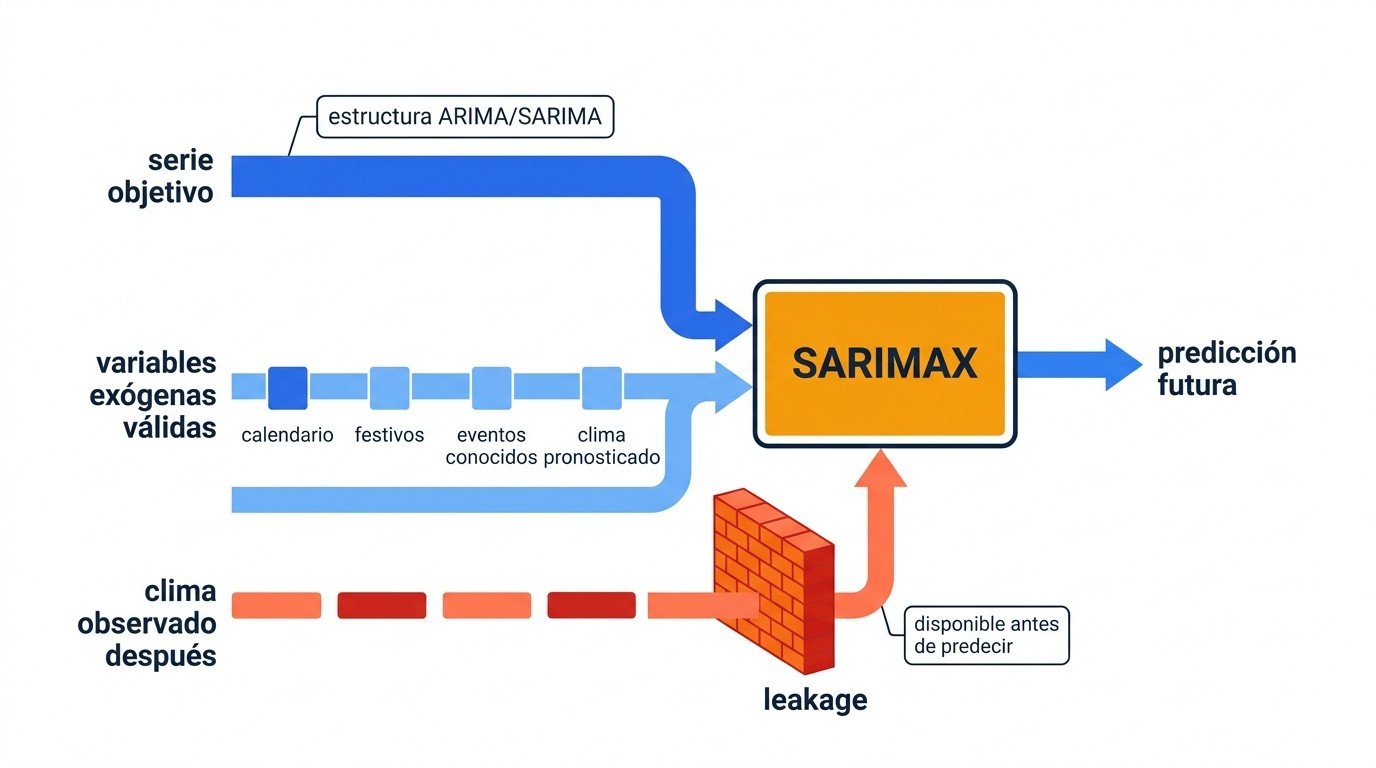
\includegraphics[width=\linewidth]{figures/img_p091_20.jpg}
\column{0.42\paperwidth}
\begin{itemize}
\item SARIMAX agrega covariables externas a la estructura ARIMA/SARIMA.
\item Las covariables solo son válidas si existen antes de predecir.
\item Si el clima observado llega después, debe usarse pronóstico, no observación futura.
\end{itemize}
\begin{rulebox}[Regla]
Exógena futura no disponible $=$ leakage.
\end{rulebox}
\end{columns}
\end{frame}

\figframe{figures/img_p091_20.jpg}

\figframe{figures/img_p093_21.jpg}

\begin{frame}[plain]
\begin{columns}[c]
\column{0.55\paperwidth}
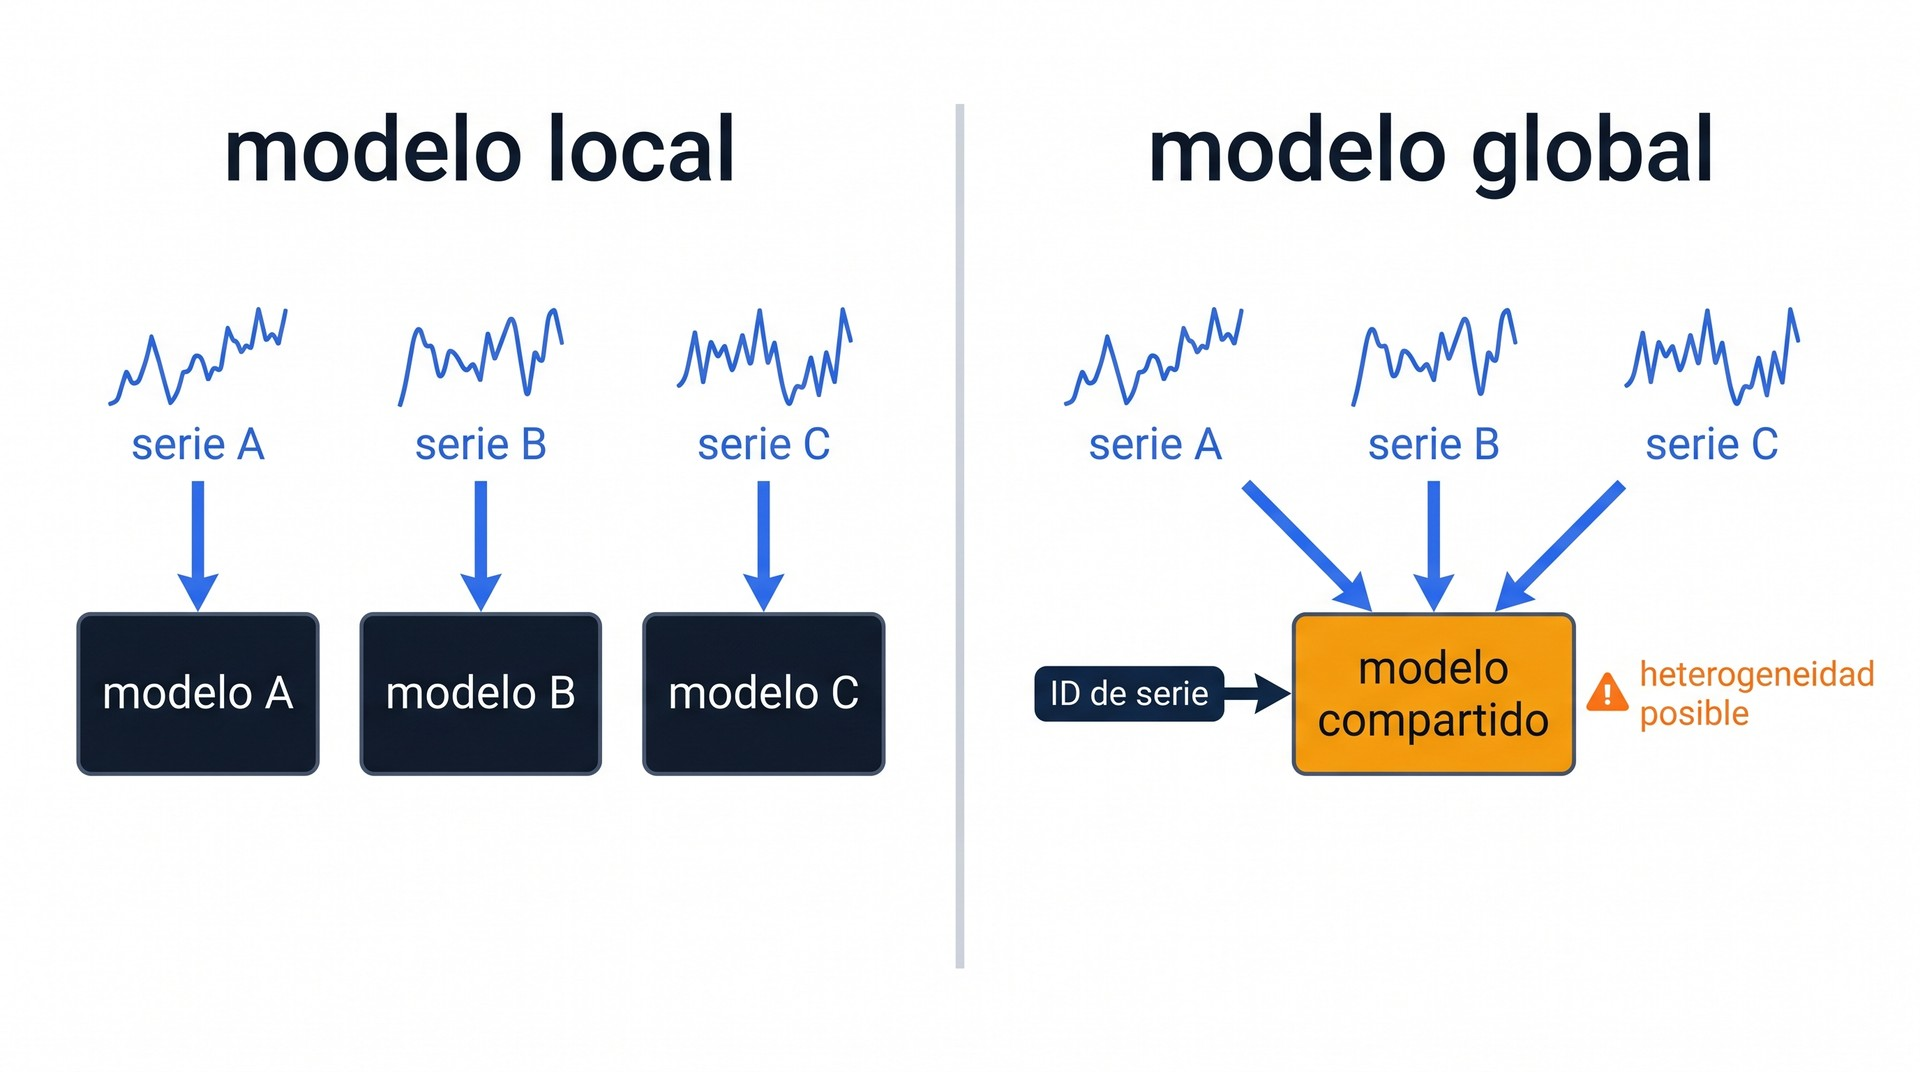
\includegraphics[width=\linewidth]{figures/img_p094_22.jpg}
\column{0.37\paperwidth}
\begin{itemize}
\item Un modelo local aprende una sola serie.
\item Un modelo global aprende patrones compartidos entre varias series.
\item La identidad de la serie debe estar representada si el modelo mezcla comportamientos.
\end{itemize}
\begin{center}
Aquí lo tratamos como concepto; la implementación multiserie completa queda fuera del núcleo.
\end{center}
\end{columns}
\end{frame}

\figframe{figures/img_p094_22.jpg}

% ============================================================ p96
\subsection{Del criterio metodológico al experimento reproducible}
\sectionframe{\LARGE Del criterio metodológico al\\experimento reproducible}

\begin{frame}{El notebook ejecuta el contrato metodológico}
\framesubtitle{NB03 debe ejecutar sin romper la disponibilidad temporal}
\bigstate{El notebook no decide el método; ejecuta el contrato metodológico definido en clase.}
\begin{columns}[T]
\column{0.47\textwidth}
\textbf{Las slides fijan}
\begin{itemize}
\item target temporal;
\item horizonte;
\item features válidas;
\item validación temporal;
\item lectura de métricas.
\end{itemize}
\column{0.47\textwidth}
\textbf{El notebook ejecuta}
\begin{itemize}
\item alineación de filas;
\item lags y rolling windows;
\item baselines temporales;
\item walk-forward validation;
\item MAE, RMSE, MASE y multi-horizon.
\end{itemize}
\end{columns}
\end{frame}

\figframe{figures/img_p098_23.jpg}

\begin{frame}[fragile]{Pseudocódigo: target, features y validación}
\framesubtitle{La implementación completa pertenece a NB03}
\vspace{1.5em}
\begin{lstlisting}[backgroundcolor={},numbers=left,numberstyle=\tiny\color{mlgray},commentstyle=\color{mltext}\itshape]
# 1. Ordenar por tiempo
# 2. Crear target futuro: y.shift(-horizon)
# 3. Crear features históricas: lag = y.shift(+k)
# 4. Crear rolling válido: y.shift(1).rolling(window)
# 5. Separar train y validación respetando cronología
# 6. Ajustar preprocessing solo dentro de train
# 7. Predecir bloque futuro y guardar métricas por fold
\end{lstlisting}
\begin{rulebox}[Cuidado]
Si una transformación aprende algo de validación o test antes de tiempo, el experimento deja de ser evidencia confiable.
\end{rulebox}
\end{frame}

\begin{frame}{Qué debe inspeccionarse en NB03}
\framesubtitle{No basta con que el notebook corra}
\centering
\begin{tabular}{@{}l P{0.6\textwidth}@{}}
\toprule
\hrow \textbf{Salida del notebook} & Pregunta que debe responder\\
\midrule
\textbf{Dummy manual} & ¿la alineación entre lag y target futuro es visible?\\
\textbf{Serie sintética} & ¿random split infla el desempeño frente a validación temporal?\\
\textbf{Baselines} & ¿el modelo supera naïve, seasonal naïve y moving average?\\
\textbf{Walk-forward report} & ¿el desempeño es estable entre folds?\\
\textbf{MASE} & ¿el modelo agrega valor frente al baseline naïve?\\
\textbf{Multi-horizon} & ¿el error se degrada en 1, 3, 6 y 24 horas?\\
\bottomrule
\end{tabular}

\vspace{0.6em}
Un notebook pedagógico no termina en una tabla de métricas: termina en una interpretación defendible.
\end{frame}

% ============================================================ p101
\subsection{Demo aplicada: Metro Interstate Traffic Volume}
\sectionframe{\LARGE Demo aplicada: Metro Interstate\\Traffic Volume}

\begin{frame}{La historia aplicada de la demo}
\framesubtitle{De una autopista horaria a un experimento temporal defendible}
\centering
\begin{tabular}{@{}l l@{}}
\toprule
\hrow \textbf{Componente} & Decisión de la demo\\
\midrule
\textbf{Target} & volumen de tráfico futuro\\
\textbf{Momento de predicción} & cada hora disponible en la serie\\
\textbf{Horizonte principal} & $h = 1$ hora adelante\\
\textbf{Horizontes secundarios} & $h \in \{3, 6, 24\}$\\
\textbf{Features} & lags, rolling windows, calendario, clima disponible\\
\textbf{Baselines} & naïve, seasonal naïve, moving average\\
\textbf{Modelos} & Ridge Regression e HistGradientBoostingRegressor\\
\textbf{Validación} & holdout temporal y walk-forward validation\\
\bottomrule
\end{tabular}
\end{frame}

\figframe{figures/img_p103_24.jpg}

\begin{frame}{Qué debe demostrar la demo}
\framesubtitle{No basta con entrenar Ridge y HGBR}
\bigstate{La demo debe mostrar que el resultado cambia cuando cambia el protocolo de validación.}
\begin{enumerate}
\item Random split como anti-ejemplo.
\item Temporal holdout como primera corrección.
\item Walk-forward como evaluación más operacional.
\item Baselines temporales antes de modelos supervisados.
\item Error por horizonte antes de una conclusión final.
\end{enumerate}
\begin{center}
El mejor modelo no es el que gana en un split cómodo, sino el que mejora referencias honestas bajo un protocolo temporal defendible.
\end{center}
\end{frame}

% ============================================================ p105
\section{Checklist temporal y cierre metodológico}
\sectionframe{\LARGE Checklist temporal y cierre\\metodológico}

\imageframe{figures/img_p106_25.jpg}

\begin{frame}{Un resultado temporal defendible es una cadena}
\framesubtitle{Si falta un eslabón, el score pierde credibilidad}
\begin{center}\large Un modelo temporal no se defiende por tener bajo error.\\[0.3em]
Se defiende porque target, horizonte, features, baseline, validación, leakage y métrica forman un argumento coherente.\end{center}
\begin{columns}[T]
\column{0.47\textwidth}
\textbf{Evidencia fuerte}
\begin{itemize}
\item target y horizonte explícitos;
\item features disponibles en $t$;
\item baseline temporal superado;
\item walk-forward sin contaminación.
\end{itemize}
\column{0.47\textwidth}
\textbf{Evidencia frágil}
\begin{itemize}
\item random split sin justificación;
\item rolling windows mal alineadas;
\item preprocessing antes del split;
\item un único score para todos los horizontes.
\end{itemize}
\end{columns}
\end{frame}

% ============================================================ p108
\subsection{Apéndice}
\sectionframe{\LARGE Apéndice}

\begin{frame}{Glosario}
\framesubtitle{Términos que deben usarse con precisión}
\centering\footnotesize
\begin{tabular}{@{}l P{0.64\textwidth}@{}}
\toprule
\hrow \textbf{Término} & Interpretación operativa\\
\midrule
\textbf{Momento de predicción} $t$ & instante desde el cual el sistema debe decidir usando información disponible\\
\textbf{Horizonte} $h$ & distancia entre el momento de predicción y el target futuro\\
$X_t$ & conjunto de features construidas con información disponible hasta $t$\\
\textbf{Lag} & valor histórico usado como memoria puntual\\
\textbf{Rolling window} & resumen de una ventana histórica, si mira solo hacia atrás\\
\textbf{Walk-forward} & evaluación que avanza cronológicamente entrenando en pasado y validando en futuro\\
\textbf{MASE} & error relativo al baseline naïve; mide si el modelo agrega valor temporal\\
\bottomrule
\end{tabular}
\end{frame}

\figframe{figures/img_p110_26.jpg}

\begin{frame}{Diagnóstico rápido de invalidez}
\framesubtitle{Cinco preguntas antes de creer el resultado}
\begin{rulebox}[{\normalsize Un experimento temporal es frágil si responde mal a cualquiera de estas preguntas}]
\setbeamercolor{enumerate item}{fg=mlred}
\begin{enumerate}
\item ¿El target futuro está claramente alineado con el momento de predicción?
\item ¿Cada feature existía en el momento $t$?
\item ¿El preprocessing fue ajustado solo con entrenamiento?
\item ¿La validación respeta la dirección del tiempo?
\item ¿El modelo supera un baseline temporal honesto?
\end{enumerate}
\vspace{0.3em}
\end{rulebox}
\vspace{1em}
\begin{center}
Si una respuesta depende de mirar el futuro, el resultado ya no es evidencia temporal confiable.
\end{center}
\end{frame}

\figframe{figures/img_p112_27.jpg}

\begin{frame}{Diferenciación como nota opcional}
\framesubtitle{A veces el modelo debe aprender variaciones, no valores absolutos}
\vspace{1.5em}
{\Large\[ \nabla y_t = y_t - y_{t-1} \qquad \nabla_s y_t = y_t - y_{t-s} \]}
\begin{columns}[T]
\column{0.47\textwidth}
\textbf{Diferencia regular}
\begin{itemize}
\item reduce tendencia;
\item trabaja con cambios consecutivos;
\item aparece en ARIMA como $d$.
\end{itemize}
\column{0.47\textwidth}
\textbf{Diferencia estacional}
\begin{itemize}
\item reduce ciclos repetidos;
\item compara contra $s$ pasos atrás;
\item aparece en SARIMA como $D$.
\end{itemize}
\end{columns}
\end{frame}

\begin{frame}{Mini-casos para cierre o discusión}
\framesubtitle{Úselos si queda tiempo o como preparación para examen}
\begin{taskbox}[{\large Decida si el diseño es defendible}]
Para cada caso, indique qué parte del protocolo aceptaría, qué parte corregiría y qué evidencia pediría antes de creer el score.
\end{taskbox}
\begin{enumerate}\small
\item Un modelo de ventas usa random split porque tiene cinco años de datos.
\item Un modelo de tráfico reporta bajo MAE a 1 hora, pero no evalúa 24 horas.
\item Un modelo de demanda supera Ridge, pero no supera seasonal naïve.
\item Un modelo fisiológico usa variables calculadas con toda la estancia del paciente.
\item Un PI con sensores secuenciales no define horizonte, pero ya compara modelos.
\end{enumerate}
\begin{goldbox}[Respuesta esperada]
La discusión debe empezar por disponibilidad, horizonte, baseline y validación; no por el nombre del algoritmo.
\end{goldbox}
\end{frame}

\begin{frame}{Cómo esta sesión alimenta el taller modular}
\framesubtitle{La lógica temporal también entrena criterio para problemas supervisados reales}
\centering
\begin{tabular}{@{}l P{0.45\textwidth}@{}}
\toprule
\hrow \textbf{Aprendizaje de hoy} & Cómo se transfiere al taller\\
\midrule
\textbf{Definir target y horizonte} & formular con precisión qué se predice y cuándo se decide\\
\textbf{Auditar disponibilidad de features} & evitar leakage antes de celebrar métricas\\
\textbf{Comparar contra baselines} & demostrar valor frente a referencias simples y honestas\\
\textbf{Validar con protocolo correcto} & escoger un esquema compatible con el tipo de dato\\
\textbf{Interpretar métricas con contexto} & cerrar con una decisión defendible, no solo con una tabla\\
\bottomrule
\end{tabular}

\vspace{0.4em}
El taller no mide si el código corre únicamente; mide si la evaluación sostiene una decisión.
\end{frame}

\begin{frame}{Preguntas de revisión para examen y PI}
\framesubtitle{La evaluación buscará decisiones correctas, no trivia de librerías}
\begin{taskbox}[{\large Responda sin entrenar todavía}]
Si un proyecto tiene mediciones secuenciales o predicción hacia futuro, el equipo debe justificar estas decisiones.
\end{taskbox}
\begin{enumerate}\small
\item ¿Cuál es exactamente el target temporal?
\item ¿Desde qué momento se predice y cuál es el horizonte?
\item ¿Qué features existían realmente en el momento $t$?
\item ¿Qué baseline temporal debe ser superado?
\item ¿Qué split respeta la cronología del fenómeno?
\item ¿Dónde podría entrar leakage antes del modelo?
\item ¿La métrica responde a la decisión operativa?
\item ¿El error se reporta por horizonte cuando corresponde?
\end{enumerate}
\end{frame}

\begin{frame}{Lo que debe quedar claro}
\framesubtitle{La temporalidad no es decoración del dataset}
\Lg
\begin{itemize}
\item Si el problema tiene tiempo, el futuro no puede ayudar a entrenar, transformar, seleccionar o validar el pasado.
\item La confianza nace cuando el experimento respeta esa dirección.
\item Un resultado temporal solo merece confianza si target, horizonte, disponibilidad de información, baseline, validación, métricas y decisión operativa están alineados.
\end{itemize}
\end{frame}

\begin{frame}{Transición a la siguiente sesión}
\framesubtitle{Después del tiempo aparecen usuarios, ítems, interacciones y rankings}
\begin{center}\large
Hoy rompimos la idea de que las filas son intercambiables cuando existe tiempo.\\[0.8em]
En la próxima sesión, romperemos otra intuición: no siempre queremos predecir un único valor, a veces queremos ordenar opciones para una persona.\\[1.4em]
El curso sigue alejándose del tabular simple: primero apareció el tiempo; ahora aparecerán preferencias, utilidad, recomendación y evaluación top-N.
\end{center}
\end{frame}

% ============================================================ p119
\begin{frame}[plain]
\begin{tikzpicture}[remember picture,overlay]
\node[anchor=north west,inner sep=0] at ([xshift=309bp,yshift=-45bp]current page.north west)
  {
\includegraphics[width=117bp,height=78bp]{figures/img_p119_28.jpg}};
\node[anchor=north west,inner sep=0] at ([xshift=177bp,yshift=-191bp]current page.north west)
  {
\includegraphics[width=96bp,height=64bp]{figures/img_p119_29.jpg}};
\node[anchor=center,align=center] at ([xshift=160bp,yshift=-86bp]current page.north west)
  {{\color{mltitle}\huge\bfseries Gracias por su atención}\\[0.5em]
   {\color{mltitle}\large ¿Preguntas, comentarios o discusión?}};
\node[anchor=center,align=center,font=\small] at ([xshift=227bp,yshift=-165bp]current page.north west)
  {\textbf{Aprendizaje Automático}\\
   SI7009 · Universidad EAFIT};
\end{tikzpicture}
\end{frame}

\end{document}
